\documentclass[12pt,a4paper]{report}

\usepackage[utf8]{inputenc}
\usepackage[T1]{fontenc}
\usepackage{geometry}
\usepackage{graphicx}
\usepackage{booktabs}
\usepackage{float}
\usepackage{hyperref}
\usepackage{xcolor}
\usepackage{array}
\usepackage{longtable}
\usepackage{ifthen}

\geometry{margin=1in}
\graphicspath{{../results/benchmark/plots/}}

\hypersetup{
    colorlinks=true,
    linkcolor=black,
    urlcolor=blue,
    citecolor=black
}

\begin{document}

\begin{titlepage}
    \centering
    \vspace*{1.2cm}

    \IfFileExists{unipi_logo.png}{
        
\includegraphics[width=0.28\textwidth]{unipi_logo.png}\\[0.8cm]
    }{
        {\Large\color{blue!35!black}\textsc{In Supremae Dignitatis}}\\[-0.1cm]
        {\large\color{blue!35!black}\textsc{1343}}\\[0.8cm]
    }

    {\Huge\color{blue!35!black}\textsc{Universit\`a di Pisa}}\\[1.6cm]

    {\Large Artificial Intelligence and Data Engineering}\\[0.35cm]
    {\Large Cloud Computing}\\[1.8cm]

    {\huge\bfseries Project Documentation}\\[1.8cm]

    {\Large Author:}\\[0.25cm]
    {\Large Zeynaddin Papakhov}\\[1.4cm]

    {\large Academic Year: 2025--2026}\\[0.5cm]
    {\large Wikimedia Pageview Analytics with Hadoop MapReduce}

    \vfill
\end{titlepage}

\tableofcontents
\newpage

\chapter{Introduction}

\section{Application Scenario}

Modern web platforms generate large volumes of access events every hour. Each user request, page visit, and automated access can be recorded as a log-like event that describes what was requested and how frequently it was accessed. Wikimedia projects represent a realistic example of this scenario, since their public pageview dumps contain large-scale hourly traffic information across many languages, projects, and pages.

The application scenario of this project is a batch web-traffic analytics pipeline for Wikimedia Pageviews data. The system is designed to ingest raw pageview files, transform them into structured records, and compute aggregate indicators that summarize the behavior of the traffic over a selected time window.

The target users of this type of application are data engineers, system administrators, and analysts who need to understand which projects and pages receive the highest traffic and how traffic changes over time. The workload is suitable for cloud-oriented data processing because it consists of many independent records that can be parsed and aggregated in parallel.

\section{Analytics Workflow}

The application computes four main analytical outputs:

\begin{itemize}
    \item \textbf{Total traffic volume}: the total number of views in the selected time window.
    \item \textbf{Project ranking}: the top Wikimedia projects by number of views.
    \item \textbf{Page ranking}: the top pages by number of views, represented as \texttt{project|page}.
    \item \textbf{Hourly traffic trend}: the total number of views grouped by hour.
\end{itemize}

This workflow combines parsing, filtering, aggregation, ranking, and time-based statistics extraction. It is intentionally more complex than a single counter because the page-level ranking may involve millions of distinct keys. This high-cardinality component is also what makes the workload interesting from a scalability perspective.

\section{The Distributed Processing Workflow}

The distributed workflow is divided into the following stages:

\begin{enumerate}
    \item \textbf{Data ingestion}: hourly Wikimedia Pageviews files are collected and uploaded to HDFS.
    \item \textbf{Parsing and cleaning}: raw text lines are parsed into structured records. Malformed records and non-positive view counts are discarded.
    \item \textbf{Intermediate representation}: valid records are serialized into a custom Hadoop Writable and written as SequenceFiles.
    \item \textbf{Metric generation}: structured records are transformed into analytical keys such as \texttt{TOTAL\_VIEWS}, \texttt{PROJECT:<project>}, \texttt{PAGE:<project>|<page>}, and \texttt{HOUR:<hour>}.
    \item \textbf{Shuffle and aggregation}: Hadoop redistributes intermediate key-value pairs to reducers, where partial values are summed.
    \item \textbf{Result generation}: the final reducer output is written as JSON-like summaries containing totals, rankings, and hourly statistics.
\end{enumerate}

The same analytical objective is implemented in a Python sequential baseline. This baseline is used as a non-parallel reference point for performance comparison.

\chapter{Dataset description}

The dataset used in this project is the Wikimedia Pageviews dataset. It is publicly available from the Wikimedia dumps service and contains hourly pageview records for Wikimedia projects. Each input file corresponds to one hour of traffic.

A typical input record follows the structure:

\begin{verbatim}
project page_title view_count response_size
\end{verbatim}

Only the first three fields are used by the analytics pipeline. The response size field is present in the raw data but is not required for the selected analytical objectives.

The dataset was selected for three main reasons. First, it is a real web dataset rather than a synthetic benchmark. Second, it naturally supports time-window analysis because it is organized by hour. Third, it contains a high number of distinct projects and pages, making it appropriate for ranking and aggregation workloads.

The experiments use consecutive hourly files from one day. The following configurations were used:

\begin{table}[H]
\centering
\begin{tabular}{lrrrr}
\toprule
Subset & Files & Compressed & Decompressed Text & HDFS Storage \\
\midrule
1h & 1 & 51.7 MiB & 185.6 MiB & 103.5 MiB \\
4h & 4 & 199.9 MiB & 723.2 MiB & 399.8 MiB \\
8h & 8 & 400.6 MiB & 1.42 GiB & 801.3 MiB \\
16h & 16 & 845.4 MiB & 2.97 GiB & 1.7 GiB \\
\bottomrule
\end{tabular}
\caption{Dataset sizes used in the experiments. HDFS storage includes replication factor 2.}
\end{table}

The original files are stored as gzip-compressed Wikimedia hourly dumps. Hadoop stores these compressed files in HDFS, but during MapReduce execution it reads the decompressed text records. Therefore, the decompressed size better represents the logical amount of text processed by the jobs, while the HDFS storage column represents the physical space used by HDFS replication.

During the ETL phase, every valid input line is transformed into a structured record containing:

\begin{itemize}
    \item the Wikimedia project identifier;
    \item the page title;
    \item the hour extracted from the input filename;
    \item the number of views.
\end{itemize}

\chapter{Architecture Description}

The system is deployed on a single virtual machine configured with Hadoop in pseudo-distributed mode. In this configuration, Hadoop daemons such as HDFS NameNode, HDFS DataNode, YARN ResourceManager, and YARN NodeManager run on the same VM. This setup follows the single-node Hadoop cluster model and allows MapReduce jobs to be executed through the Hadoop ecosystem without requiring multiple physical machines.

\section{Data Storage and Computation Flow}

The raw input files are stored in HDFS for the Hadoop MapReduce implementation. HDFS provides the storage layer used by the MapReduce jobs. The sequential baseline, instead, reads the same files directly from the local filesystem.

The computation flow is structured as follows:

\begin{enumerate}
    \item input files are prepared locally on the VM;
    \item Hadoop input files are uploaded to HDFS under \texttt{/user/hadoop/single\_project/input/};
    \item the first MapReduce job reads the HDFS input and writes structured SequenceFile output to an intermediate HDFS directory;
    \item the second MapReduce job reads the intermediate SequenceFiles and writes the final analytics output to HDFS;
    \item benchmark scripts collect execution time and memory-related metrics and save them as CSV files.
\end{enumerate}

This architecture is important when interpreting the results. Since all services run on one VM, the system does not benefit from true multi-node data locality or distributed hardware parallelism. Nevertheless, Hadoop still performs job scheduling, container allocation, HDFS I/O, intermediate writes, and shuffle operations. These overheads explain why Hadoop is slower than the sequential baseline for smaller completed datasets.

\section{Project Structure}

The project is organized into the following main directories:

\begin{itemize}
    \item \texttt{hadoop-pageviews/}: Java Hadoop implementation and Maven configuration;
    \item \texttt{sequential/}: Python sequential baseline;
    \item \texttt{scripts/}: dataset preparation, HDFS upload, benchmark, fetch, and plot scripts;
    \item \texttt{results/benchmark/}: CSV benchmark results and generated plots;
    \item \texttt{docs/}: LaTeX documentation and generated PDF report.
\end{itemize}

\chapter{Implementation}

\section{Hadoop}

\subsection{Implementation Choices and Optimizations}

The Hadoop implementation consists of two non-iterative MapReduce jobs in cascade, both written in Java.

\begin{itemize}
    \item \textbf{Job 1: ETL}. The first job parses raw Wikimedia Pageviews lines, filters invalid records, extracts the hour from the input filename, and writes structured records as SequenceFiles.
    \item \textbf{Job 2: Analytics}. The second job reads the structured intermediate records and computes the final aggregate statistics.
\end{itemize}

Several Hadoop-specific features were implemented:

\begin{itemize}
    \item \textbf{Custom Writable}: a \texttt{PageviewRecord} class is used to pass structured records between the ETL and analytics jobs. This avoids fragile string concatenation and makes the intermediate format typed and explicit.
    \item \textbf{setup() method}: the ETL mapper uses \texttt{setup()} to extract the hour from the input filename once per map task.
    \item \textbf{cleanup() method}: the analytics mapper uses \texttt{cleanup()} to emit locally aggregated metrics only at the end of the map task.
    \item \textbf{In-mapper combining}: the analytics mapper stores partial sums in a local hash map. This reduces the number of emitted key-value pairs and decreases shuffle pressure.
    \item \textbf{Custom partitioning}: a \texttt{MetricsPartitioner} routes metrics according to their semantic category, such as project, page, hour, or total.
    \item \textbf{Multiple reducers}: the implementation accepts the number of reducers as a command-line parameter. The experiments evaluate 1, 2, 4, and 8 reducers.
\end{itemize}

The top-project and top-page outputs are limited to the top 10 entries. This keeps the output readable and prevents the reducer from storing unnecessary result entries.

\subsection{MapReduce workflow pseudocode}

\textbf{Algorithm 1: PageviewRecord Custom Writable}

\begin{verbatim}
Class PageviewRecord implements Writable
    variables:
        project : String
        page    : String
        hour    : String
        views   : long

    write(out):
        serialize project, page, hour, views

    readFields(in):
        deserialize project, page, hour, views
\end{verbatim}

\textbf{Algorithm 2: ETL Mapper}

\begin{verbatim}
setup(context):
    inputHour = extract hour from current input filename

map(offset, line):
    fields = split line into project, page, views, responseSize
    if fields are malformed:
        skip line
    if views cannot be parsed or views <= 0:
        skip line

    record = PageviewRecord(project, page, inputHour, views)  // responseSize is ignored
    emit(NullWritable, record)
\end{verbatim}

\textbf{Algorithm 3: Analytics Mapper with In-Mapper Combining}

\begin{verbatim}
setup(context):
    metricsCache = empty hash map

map(_, record):
    metricsCache["TOTAL_VIEWS"] += record.views
    metricsCache["PROJECT:" + record.project] += record.views
    metricsCache["PAGE:" + record.project + "|" + record.page] += record.views
    metricsCache["HOUR:" + record.hour] += record.views

cleanup(context):
    for each (metricKey, partialSum) in metricsCache:
        emit(metricKey, partialSum)
\end{verbatim}

\textbf{Algorithm 4: Metrics Partitioner}

\begin{verbatim}
getPartition(metricKey, value, numReducers):
    if metricKey contains ":":
        prefix = substring before ":"
    else:
        prefix = metricKey
    return hash(prefix) modulo numReducers
\end{verbatim}

\textbf{Algorithm 5: Analytics Reducer}

\begin{verbatim}
reduce(metricKey, values):
    sum = total of all values

    if metricKey == "TOTAL_VIEWS":
        update global total
    else if metricKey starts with "PROJECT:":
        update project ranking candidates
    else if metricKey starts with "PAGE:":
        update page ranking candidates
    else if metricKey starts with "HOUR:":
        update hourly totals

cleanup(context):
    write JSON summary:
        total views
        top projects
        top pages
        views by hour
\end{verbatim}

\textbf{Algorithm 6: Driver}

\begin{verbatim}
main(args):
    read reducers, input path, intermediate path, output path, topN
    configure memory limits and analytics.top.n
    delete existing intermediate and output paths

    configure Job 1:
        mapper = ETLMapper
        reducers = 0
        output = SequenceFile<PageviewRecord>
    run Job 1

    configure Job 2:
        mapper = AnalyticsMapper
        partitioner = MetricsPartitioner
        reducer = AnalyticsReducer
        reducers = user parameter
        input = SequenceFile
        output = text/JSON-like summary
    run Job 2
\end{verbatim}

\section{Sequential Baseline}

The sequential baseline is implemented in Python. It reads the same Wikimedia Pageviews files from the local filesystem and computes the same metrics using Python dictionaries and counters.

This implementation is intentionally non-parallel. It provides a control point for evaluating whether the Hadoop overhead is justified under the available hardware constraints. For small and medium completed datasets, the sequential script is faster because it avoids YARN startup, HDFS reads, intermediate writes, and shuffle. However, it stores page-level counters inside a single process, which becomes a memory limitation at larger input sizes.

\section{Requirements Coverage}

\begin{longtable}{p{0.36\textwidth}p{0.54\textwidth}}
\toprule
\textbf{Requirement} & \textbf{Project implementation} \\
\midrule
\endhead
Pseudo-distributed Hadoop VM & Hadoop runs in pseudo-distributed mode on a single VM with HDFS and YARN. \\
Autonomous dataset selection & Wikimedia Pageviews was selected and motivated as a large web analytics dataset. \\
Large dataset & The 16h stress test processes more than 100 million records and several GB of logical input. \\
Application scenario & Web traffic monitoring and pageview analytics. \\
Analytics workflow & Parsing, filtering, aggregation, ranking, and hourly trend extraction. \\
Two MapReduce jobs in cascade & Job 1 performs ETL; Job 2 performs analytics. \\
Java implementation & Both Hadoop jobs are implemented in Java. \\
In-mapper combining & The analytics mapper aggregates metrics locally and emits partial sums in \texttt{cleanup()}. \\
Custom partitioning & The custom partitioner groups metrics according to their semantic prefix. \\
setup() and cleanup() & Used in ETL and analytics mapper/reducer lifecycle methods. \\
Custom Writable & \texttt{PageviewRecord} is used as the intermediate structured record. \\
More than one reducer & The benchmarks include 1, 2, 4, and 8 reducers. \\
Python non-parallel comparison & Hadoop is compared with a sequential Python baseline. \\
Experimental evaluation & Execution time, memory usage, reducer count, and dataset size are evaluated. \\
\bottomrule
\end{longtable}

\chapter{Experimental evaluation}

\section{Default Experimental Baseline Configuration}

To keep the comparison controlled, the same analytical pipeline is executed across all configurations. The dataset-size and memory experiments use 4 Hadoop reducers. The reducer benchmark fixes the dataset at 4h and varies only the number of reducers.

The baseline configuration is summarized as follows:

\begin{itemize}
    \item \textbf{Sequential baseline}: single-threaded Python process reading local files.
    \item \textbf{Hadoop baseline}: Java MapReduce pipeline reading from HDFS and executing through YARN.
    \item \textbf{Reducer count for dataset-size benchmark}: fixed at 4 reducers.
    \item \textbf{Top-N threshold}: fixed at 10 for project and page rankings.
    \item \textbf{Correctness check}: Hadoop and sequential outputs were compared on the 1h dataset.
\end{itemize}

For the correctness check, both implementations produced the same total number of views on the 1h dataset:

\begin{center}
\begin{tabular}{lr}
\toprule
Implementation & Total Views \\
\midrule
Hadoop MapReduce & 15,459,276 \\
Sequential Python & 15,459,276 \\
\bottomrule
\end{tabular}
\end{center}

\section{Comparative Analysis of Execution Times based on Dataset Size}

To evaluate scalability, the same analytical pipeline was executed over increasing dataset sizes. Hadoop was executed with 4 reducers, while the sequential implementation processed the same files locally.

\begin{table}[H]
\centering
\begin{tabular}{lrr}
\toprule
Dataset & Hadoop 4 Reducers (s) & Sequential (s) \\
\midrule
1h & 117 & 20 \\
4h & 295 & 75 \\
8h & 583 & 154 \\
\bottomrule
\end{tabular}
\caption{Execution time by dataset size.}
\end{table}

\begin{figure}[H]
\centering
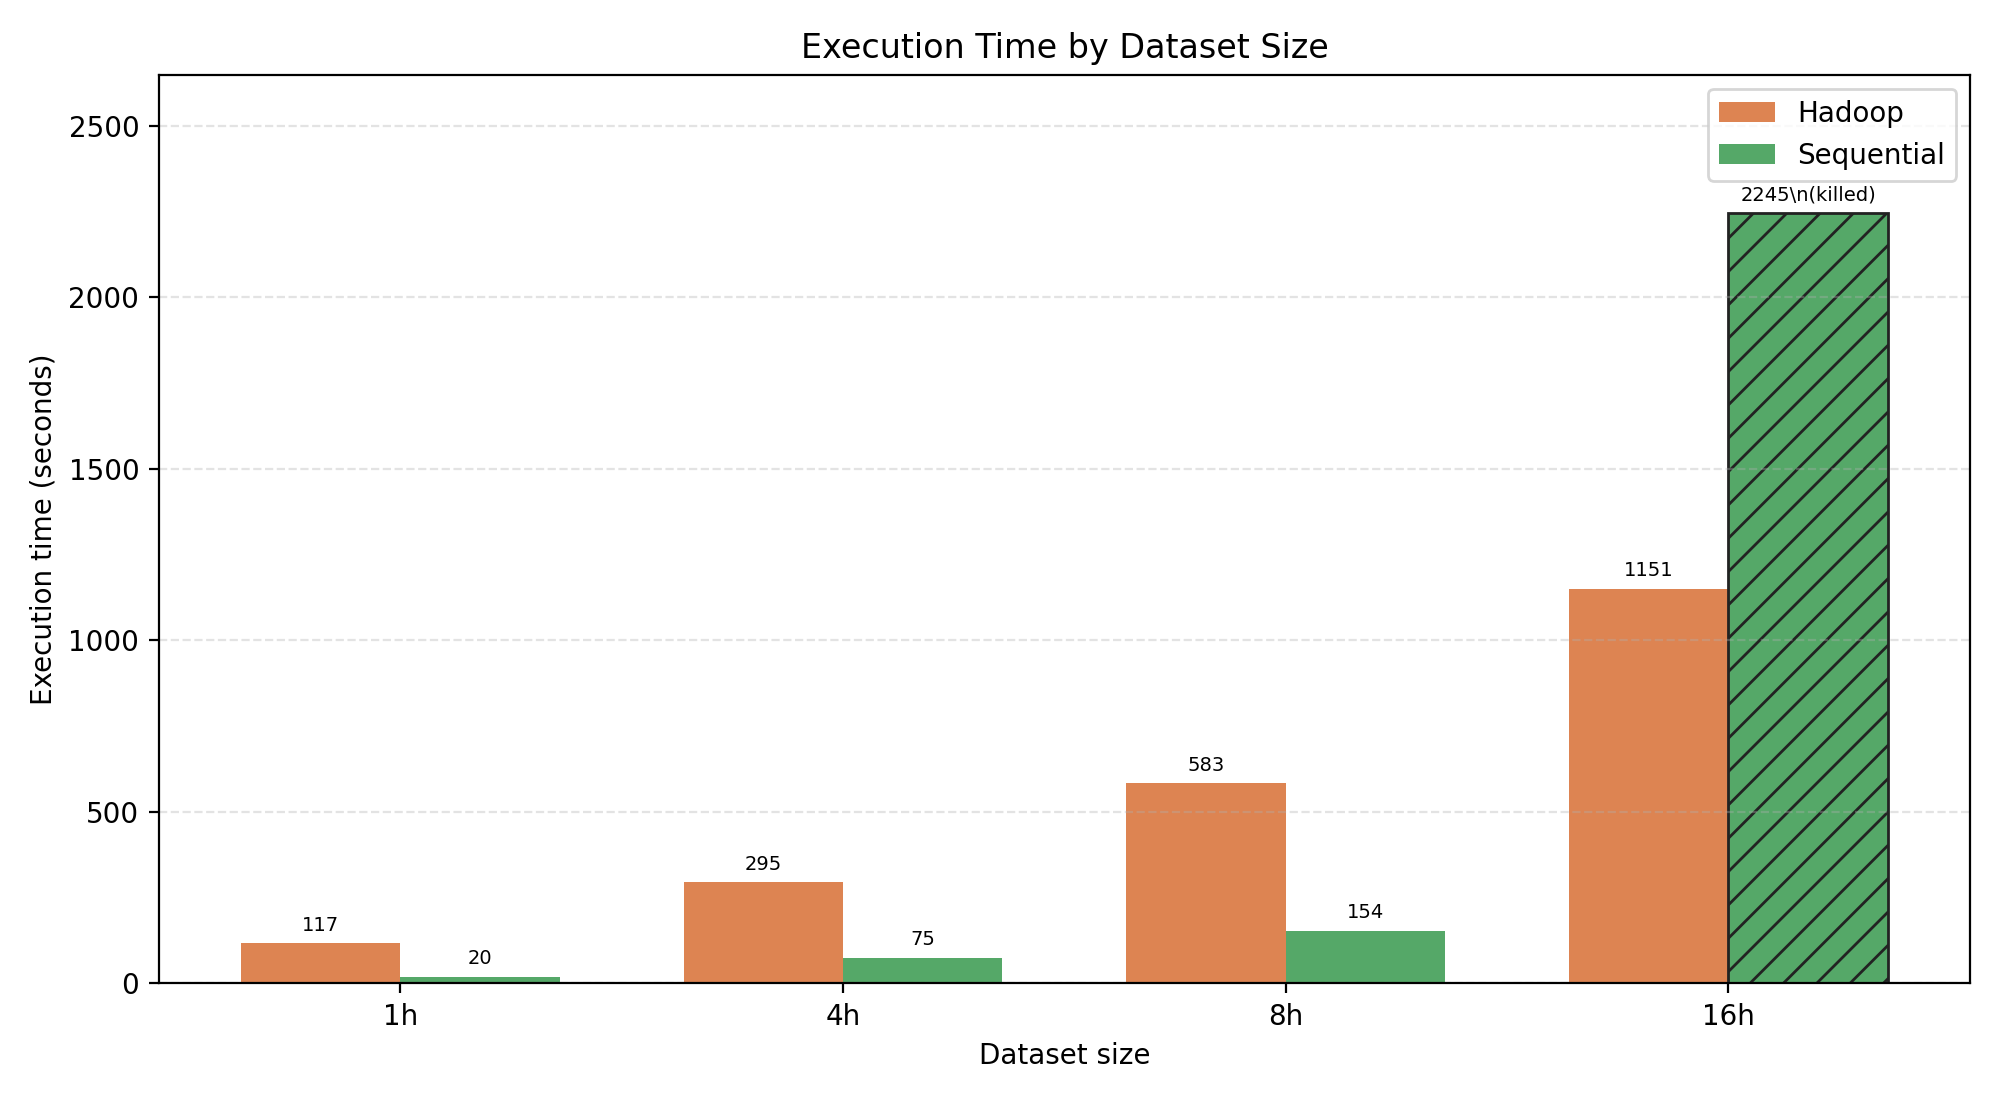
\includegraphics[width=0.95\textwidth]{execution_time_by_dataset.png}
\caption{Execution time comparison by dataset size.}
\end{figure}

The results show that the sequential baseline is faster for the completed 1h, 4h, and 8h datasets. This is expected in a single-VM pseudo-distributed environment. Hadoop pays the cost of HDFS access, YARN scheduling, intermediate materialization, and shuffle, while the sequential baseline reads files directly from local storage.

\subsection{Sequential Architecture and Memory Threshold}

The 16h stress test reveals the main limitation of the sequential approach. Hadoop completed the 16h dataset in approximately 1151 seconds, while the sequential Python process was killed after 2245 seconds.

\begin{table}[H]
\centering
\begin{tabular}{lrl}
\toprule
Implementation & Time (s) & Status \\
\midrule
Hadoop MapReduce & 1151 & Completed \\
Sequential Python & 2245 & Killed before completion \\
\bottomrule
\end{tabular}
\caption{16h stress-test behavior.}
\end{table}

The sequential process was killed because the page-level counter is stored inside a single Python process. As the number of unique pages grows, the in-memory dictionary becomes too large for the available VM memory. Hadoop, instead, is able to complete because it relies on disk-backed intermediate data, shuffle, and reducer-based aggregation.

\section{Comparative Analysis of Execution Times based on Reducers}

This experiment evaluates the impact of the number of reducers on Hadoop performance. The dataset is fixed at 4h, while the number of reducers is varied from 1 to 8.

\begin{table}[H]
\centering
\begin{tabular}{rr}
\toprule
Reducers & Hadoop Time (s) \\
\midrule
1 & 270 \\
2 & 306 \\
4 & 308 \\
8 & 319 \\
\bottomrule
\end{tabular}
\caption{Hadoop execution time by number of reducers on the 4h dataset.}
\end{table}

\begin{figure}[H]
\centering
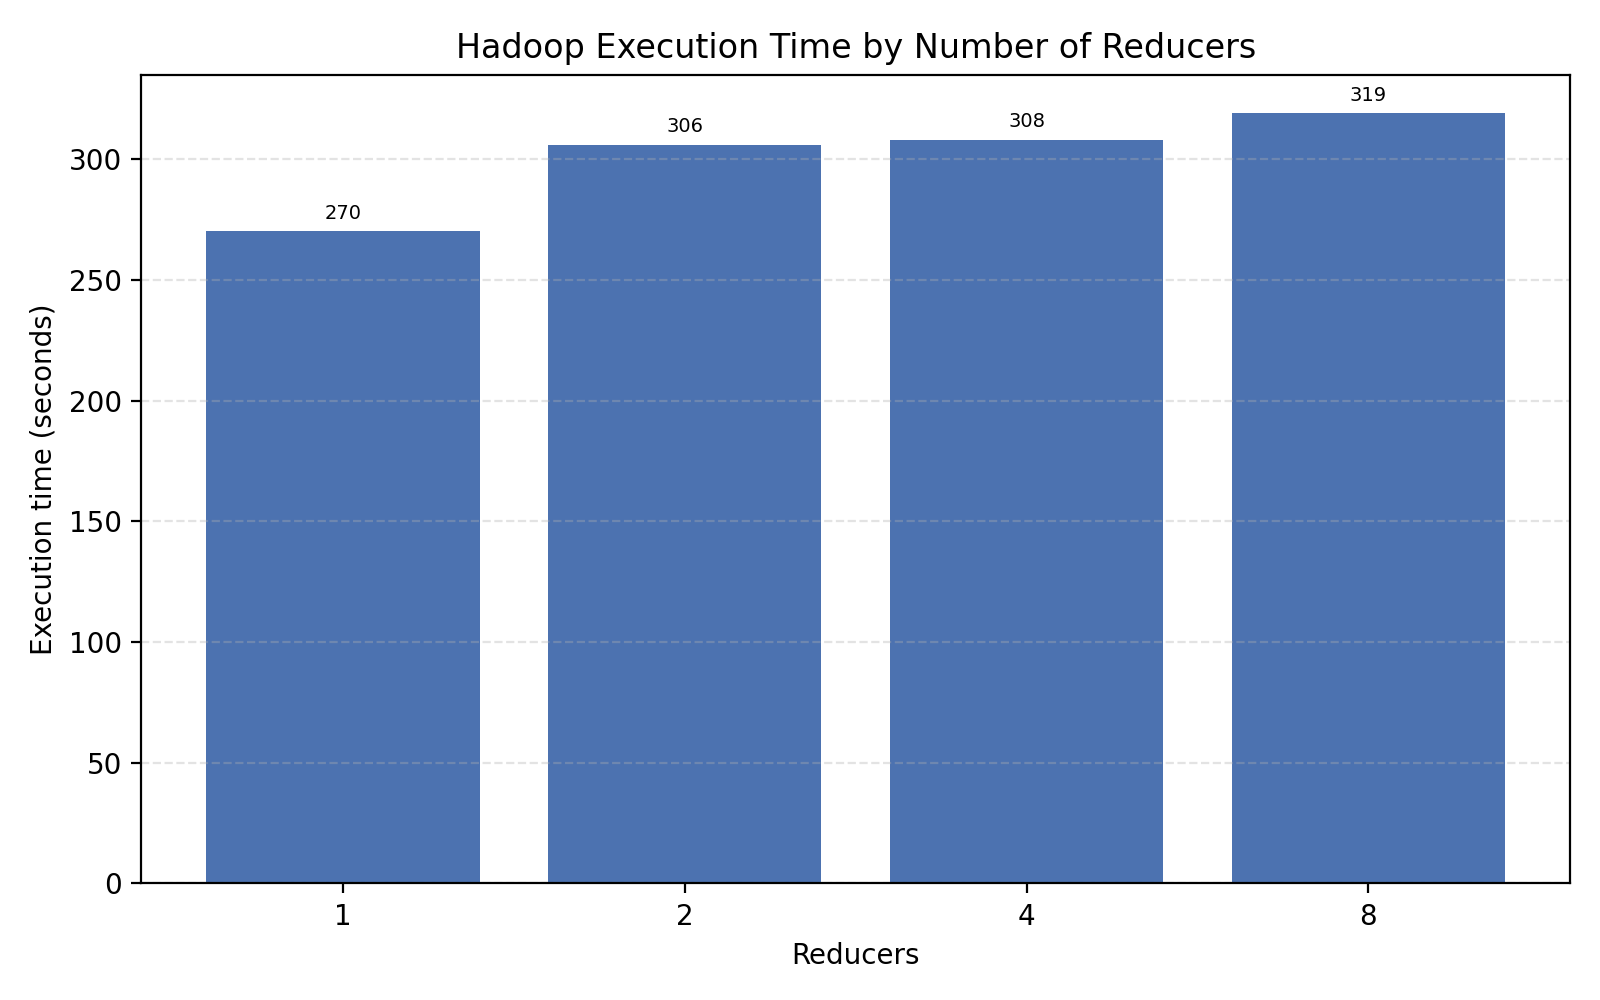
\includegraphics[width=0.85\textwidth]{execution_time_by_reducers.png}
\caption{Hadoop execution time by number of reducers.}
\end{figure}

The best runtime is obtained with one reducer. Increasing the number of reducers does not improve performance in this environment. Since the system runs on one VM, additional reducers compete for the same CPU, memory, and disk resources. The extra shuffle and scheduling overhead outweighs the potential benefit of parallel reduction.

\subsection{Hadoop Reducer Performance}

The reducer experiment indicates that the analytics job is strongly affected by framework overhead. With one reducer, the shuffle and output coordination are simpler. With more reducers, Hadoop must manage additional reduce tasks, partitioned shuffle transfers, and multiple output files. On a real multi-node cluster, more reducers could improve parallelism, but on a single VM the benefit is limited.

\section{Comparative Analysis of Memory Usage based on Dataset Size}

The memory benchmark compares Hadoop YARN allocated memory with the peak resident set size of the sequential Python process. These two metrics are not identical: Hadoop memory represents framework-managed allocation, while sequential memory represents the peak memory of a single process. Nevertheless, they show how resource pressure changes with dataset size.

\begin{table}[H]
\centering
\begin{tabular}{lrr}
\toprule
Dataset & Hadoop Avg Allocated MB & Sequential Peak RSS MB \\
\midrule
1h & 2277.53 & 991.88 \\
4h & 3051.64 & 2235.91 \\
8h & 3334.44 & 3974.96 \\
\bottomrule
\end{tabular}
\caption{Memory usage by dataset size.}
\end{table}

\begin{figure}[H]
\centering
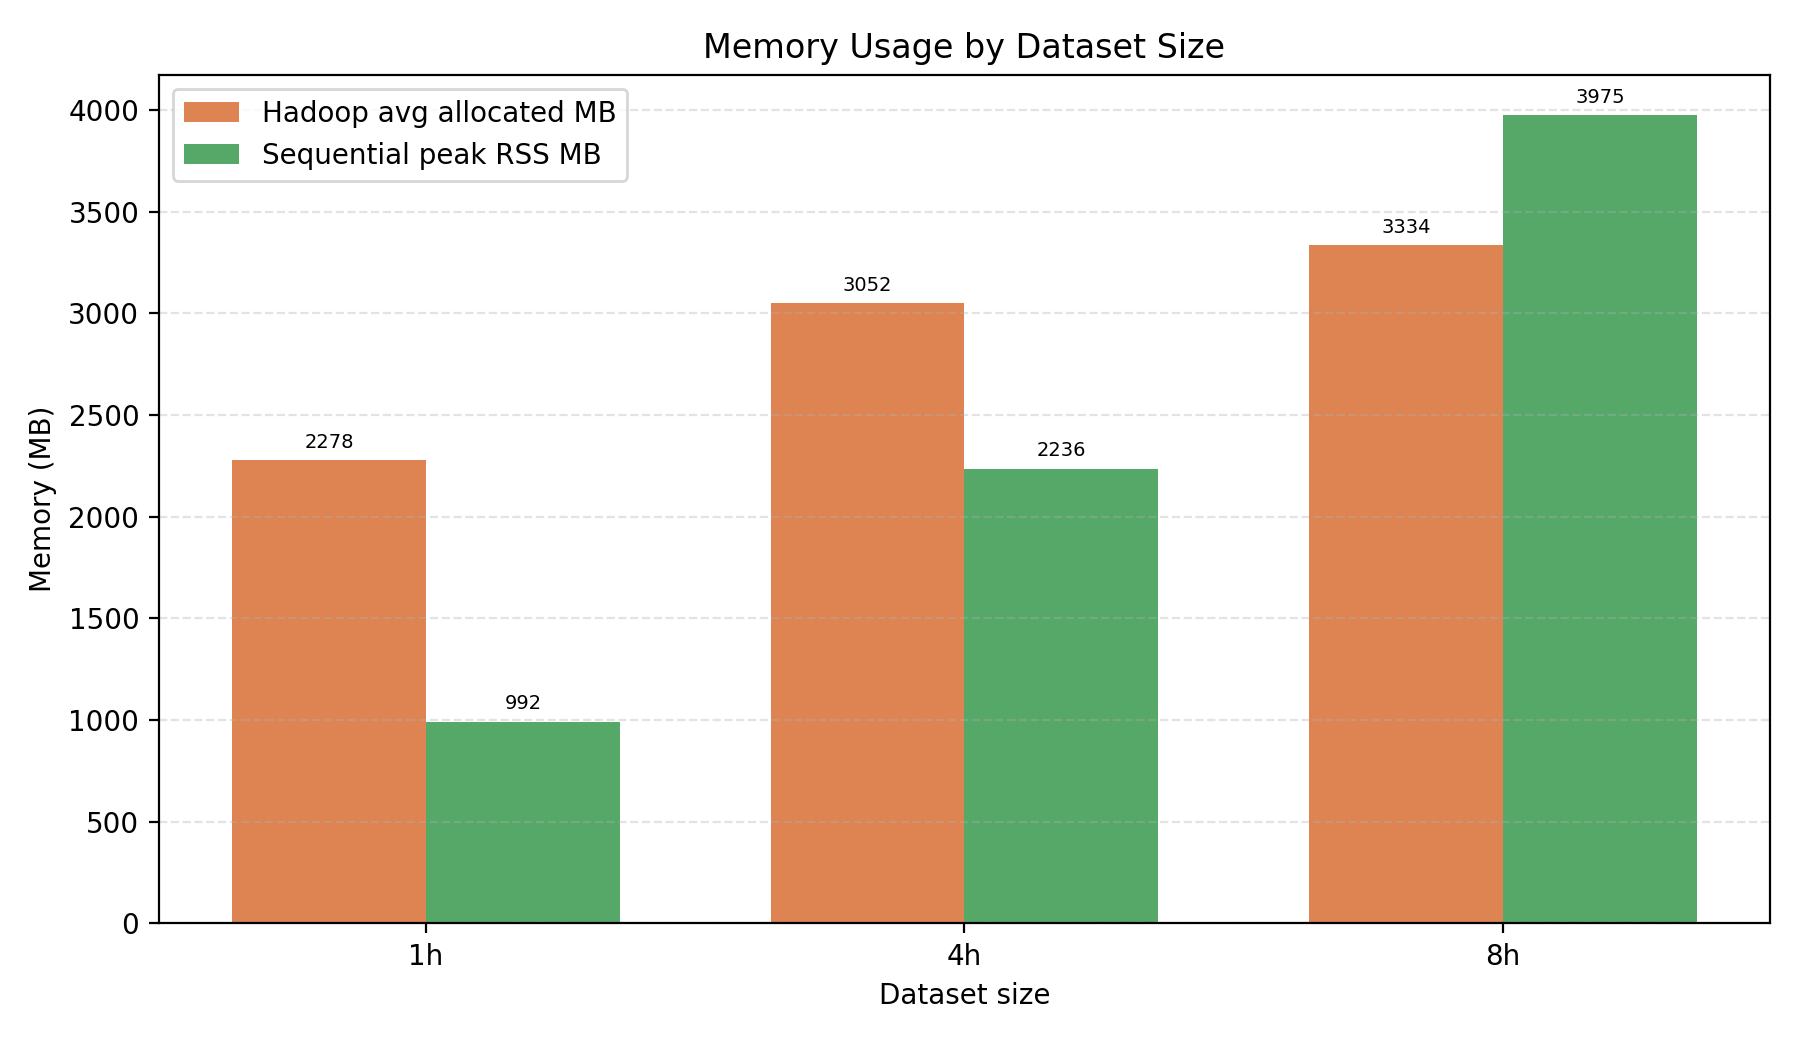
\includegraphics[width=0.95\textwidth]{memory_by_dataset.png}
\caption{Memory usage comparison by dataset size.}
\end{figure}

\subsection{Sequential Memory Behavior}

The sequential baseline shows a strong increase in memory usage as the dataset grows. This is caused by the page-level dictionary, which must keep one entry for each distinct \texttt{project|page} key. At 8h, the sequential process reaches almost 4 GB of peak RSS. At 16h, the same approach no longer completes because the process is killed due to memory pressure.

\subsection{Hadoop Memory Behavior}

Hadoop uses more memory than the sequential baseline at smaller sizes because YARN containers, map tasks, reduce tasks, and the ApplicationMaster require allocated resources. However, Hadoop's memory behavior is more stable for larger workloads because the framework spills intermediate data to disk and distributes aggregation across reduce tasks.

\subsection{Comparative Conclusion}

The results highlight a trade-off between raw speed and scalability. Sequential processing is faster while the workload fits into memory, but it eventually reaches a memory limit. Hadoop is slower in the single-VM setup, but it can complete larger workloads by relying on disk-backed distributed processing.

\chapter{Conclusion}

This project implemented a Hadoop MapReduce analytics pipeline for Wikimedia Pageviews data and compared it against a Python sequential baseline. The implementation satisfies the main project requirements: it uses two Java MapReduce jobs in cascade, a custom Writable, setup and cleanup methods, in-mapper combining, a custom partitioner, multiple reducers, and a Python non-parallel baseline.

The experiments show that the sequential baseline is faster for completed 1h, 4h, and 8h datasets because it avoids distributed framework overhead. However, the 16h stress test demonstrates the limitation of this approach: the sequential process is killed due to memory pressure, while Hadoop completes successfully.

The reducer benchmark shows that increasing the number of reducers does not automatically improve performance on a single VM. In this environment, more reducers introduce overhead rather than useful parallelism. Therefore, the results must be interpreted in the context of the pseudo-distributed setup.

Overall, Hadoop MapReduce provides better robustness for larger workloads, while the sequential baseline provides lower overhead for smaller datasets. This is the central trade-off observed in the project.

\end{document}


